\documentclass[12pt]{article}
\usepackage[utf8]{inputenc}
\usepackage[a4paper, margin=2cm]{geometry}
\usepackage{amsthm}
\usepackage{amsmath, amssymb}
\usepackage{circuitikz}
\usepackage{graphicx}
\usepackage{karnaugh-map}
\usepackage{newtxtext, newtxmath}
\usepackage{tcolorbox}
\usepackage{tikz}
\usepackage{titlesec}
\usepackage{xcolor}
\usepackage{listings}
\usepackage{xeCJK}
\definecolor{lightblue}{RGB}{135, 206, 250}
\definecolor{commentgreen}{rgb}{0.25,0.5,0.35}
\definecolor{keywordblue}{rgb}{0.13,0.13,1}
\definecolor{stringmagenta}{rgb}{0.5,0,0.35}
\tcbuselibrary{skins,theorems}

\titleformat{\section}[block]{\Large\bfseries\centering}{}{0pt}{}
\titleformat{\subsection}[block]{\bfseries}{\thesubsection}{2pt}{}

\lstdefinestyle{verilogstyle}{
  language=Verilog,                % 设置语言
  backgroundcolor=\color{white},   % 背景色
  commentstyle=\color{commentgreen},% 注释样式
  keywordstyle=\color{keywordblue}, % 关键字样式
  numberstyle=\tiny\color{gray},    % 行号的样式
  stringstyle=\color{stringmagenta},% 字符串样式
  basicstyle=\ttfamily\small,      % 代码基本样式
  breakatwhitespace=false,         % 是否只在空白处换行
  breaklines=true,                 % 自动换行
  captionpos=b,                    % 标题位置（底部）
  keepspaces=true,                 % 保留空格
  numbers=left,                    % 行号的位置
  numbersep=5pt,                   % 行号与代码的距离
  showspaces=false,                % 是否显示空格
  showstringspaces=false,          % 字符串中的空格是否显示
  showtabs=false,                  % 是否显示制表符
  tabsize=2,                       % 制表符的宽度
  frame=single,                    % 边框样式
  rulecolor=\color{black}          % 边框颜色
}

% 创建一个新的listings环境
\lstnewenvironment{verilogcode}[1][]
{
  \lstset{style=verilogstyle, #1} % 使用Verilog样式，允许自定义设置
}{}

\newtcbtheorem[no counter]{proposition}{\large\hspace{-8pt}Proposition}{
  enhanced,
  colback=white,
  colframe=lightblue,
  left=12pt,
  right=12pt,
  top=24pt,
  bottom=24pt,
  fonttitle=\bfseries
}{prop}
\newtcbtheorem[]{question}{\large\hspace{-8pt}Question :}{
  enhanced,
  colback=white,
  colframe=black,
  left=12pt,
  right=12pt,
  top=24pt,
  bottom=24pt,
  fonttitle=\bfseries
}{qst}
\newenvironment{Answer}{
  \vspace{12pt}
  {\large\textbf{\textit{\hspace{-12pt}Answer:}}}\par
  \vspace{8pt}
} {\vspace{24pt}}
\newenvironment{Proof}{
  \vspace{12pt}
  {\large\textbf{\textit{\hspace{-12pt}Proof:}}}\par
  \vspace{8pt}
} {\vspace{24pt}}

\title{DCHw1}
\author{Miki-Riako }
\date{\today}
\begin{document}

\begin{question}{}{}
  4-1 Write logic expressions and draw truth tables and analyze logic functions.
\end{question}
\begin{Answer}
\noindent\begin{minipage}{0.5\textwidth}
\begin{center}\begin{tabular}{|c|c|c|c|c|}\hline
$A$ & $B$ & $C$ & $F_1$ & $F_2$ \\ \hline
0 & 0 & 0 & 0 & 0 \\ \hline
0 & 0 & 1 & 1 & 0 \\ \hline
0 & 1 & 0 & 1 & 0 \\ \hline
0 & 1 & 1 & 0 & 1 \\ \hline
1 & 0 & 0 & 1 & 0 \\ \hline
1 & 0 & 1 & 0 & 1 \\ \hline
1 & 1 & 0 & 0 & 1 \\ \hline
1 & 1 & 1 & 1 & 1 \\ \hline
\end{tabular}\end{center}
\end{minipage}\begin{minipage}{0.5\textwidth}
由真值表易得：
\begin{align*}
  F_1=&A\oplus B\oplus C \\
  F_2=&AB+AC+BC
\end{align*}

效果：\newline

$F_1$ 为奇数有效信号校验。

$F_2$ 为检测大于等于2的有效信号。

综合一起为全加器、其中$F_2$为进位。
\end{minipage}
\end{Answer}

\begin{question}{}{}
  4-2 Write logic expressions.
\end{question}
\begin{Answer}
首先由于74LS148输入全为0。

所以输出$Y_0=Y_1=Y_2=0$。

因此，输出Y的信号取决于A。

即$Y=A$。
\end{Answer}

\begin{question}{}{}
  4-3 Analyze logic functions.
\end{question}
\begin{Answer}
首先根据当前输入情况可得：

\noindent\begin{minipage}{0.333\textwidth}
\begin{flalign*}
  Y_0&=\overline{\overline A\;\overline B} \\
  Y_1&=\overline{\overline A\;B} \\
  Y_2&=\overline{A\;\overline B} \\
  Y_3&=\overline{A\;B} \\
\end{flalign*}
\end{minipage}\begin{minipage}{0.333\textwidth}
\begin{flalign*}
  Y_0&=D_0 \\
  Y_1&=D_1 \\
  Y_2&=D_2 \\
  Y_3&=D_3 \\
\end{flalign*}
\end{minipage}\begin{minipage}{0.333\textwidth}
\begin{flalign*}
  1&=D_0\overline C\;\overline D \\
  1&=D_1\overline C\;D \\
  1&=D_2C\;\overline D \\
  1&=D_3C\;D \\
\end{flalign*}
\end{minipage}

综上
$F=\overline{\overline A\;\overline B}\;\overline C\;\overline D+\overline{\overline A\;B}\;\overline C\;D+\overline{A\;\overline B}\;C\;\overline D+\overline{A\;B}\;C\;D$。

可见，当且仅当$A=\overline C\;and\;B=\overline D$时得到有效信号。

效果即为判断A与C或B与D互反。
即判断$A=\overline C$或$B=\overline D$是否成立。

换言之，即排除$AB=CD$的情况。
\end{Answer}

\begin{question}{}{}
  4-4 Analyze logic functions.
\end{question}
\begin{Answer}
观察可得，信号仅在0（000B）以及7（111B）时输出低电平信号。

即该逻辑电路的功能为校验三输入信号是否为同有效信号。
\end{Answer}

\begin{question}{}{}
  4-9 Design Circuit: Checking odd valid signal inputs
\end{question}
\begin{Answer}
\noindent\begin{minipage}{0.5\textwidth}
\quad\quad 校验奇数个有效信号，
为异或门的基本功能。
使用异或门即可。\newline
$$F = A\oplus B\oplus C$$
\end{minipage}\begin{minipage}{0.5\textwidth}
\quad\quad 电路图如下：
\begin{center}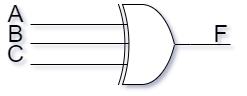
\includegraphics[width=0.5\textwidth]{image/electrical_5.png}\end{center}
\end{minipage}
\end{Answer}

\begin{question}{}{}
  4-10 Design Circuit.
\end{question}
\begin{Answer}
\noindent\begin{minipage}{0.5\textwidth}
根据题目所述，可以绘制真值表如下：
\begin{center}\begin{tabular}{|c|c|c|c|c|c|}\hline
$X_2$ & $X_1$ & $X_0$ & $F_2$ & $F_1$ & $F_0$ \\ \hline
0 & 0 & 0 & 0 & 0 & 1 \\ \hline
0 & 0 & 1 & 0 & 0 & 1 \\ \hline
0 & 1 & 0 & 1 & 0 & 0 \\ \hline
0 & 1 & 1 & 1 & 0 & 1 \\ \hline
1 & 0 & 0 & 1 & 1 & 0 \\ \hline
1 & 0 & 1 & 1 & 1 & 1 \\ \hline
1 & 1 & 0 & 0 & 0 & 0 \\ \hline
1 & 1 & 1 & 0 & 0 & 0 \\ \hline
\end{tabular}\end{center}
\end{minipage}\begin{minipage}{0.5\textwidth}
根据真值表，得到电路图如下：

\begin{center}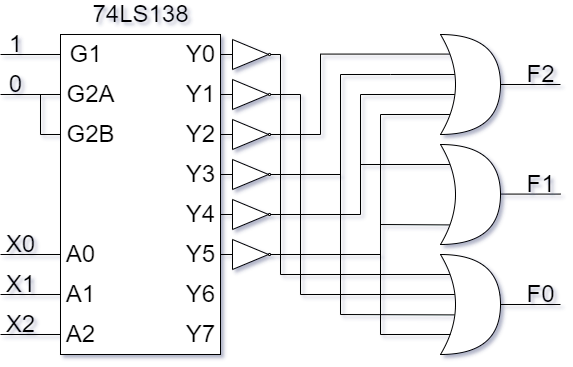
\includegraphics[width=0.8\textwidth]{image/electrical_6.png}\end{center}
\end{minipage}
\end{Answer}

\begin{question}{}{}
  4-14 Design Circuit.
\end{question}
\begin{Answer}
由于一片74LS138只能表示8个数字，
故本题需要两篇74LS138。

根据题目所述，绘制电路图如下：
\begin{center}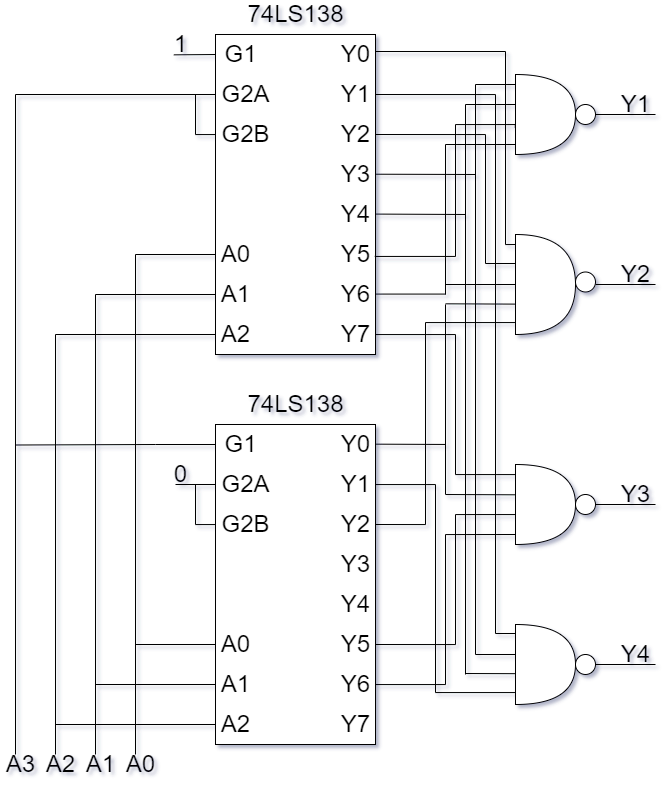
\includegraphics[width=0.5\textwidth]{image/electrical_7.png}\end{center}
\end{Answer}

\begin{question}{}{}
  4-15 Coding in Verilog.
\end{question}
\begin{Answer}
\begin{verilogcode}[caption={Verilog: 15}]
module half_add_sub(
    input A,
    input B,
    input X,
    output Si,
    output Ca,
    );
assign Si = A ^ B;
assign Ca = X ? (~A & B) : (A & B);
endmodule
\end{verilogcode}
\end{Answer}

\begin{question}{}{}
  4-16 Design Circuit.
\end{question}
\begin{Answer}
\begin{minipage}{0.5\textwidth}
根据题目所述，可以绘制真值表如下：
\begin{center}\begin{tabular}{|c|c|c|c|c|}\hline
$A$ & $B$ & $C$ & $S$ & $C_{i+1}$ \\ \hline
0 & 0 & 0 & 0 & 0 \\ \hline
0 & 0 & 1 & 1 & 1 \\ \hline
0 & 1 & 0 & 1 & 1 \\ \hline
0 & 1 & 1 & 0 & 1 \\ \hline
1 & 0 & 0 & 1 & 0 \\ \hline
1 & 0 & 1 & 0 & 0 \\ \hline
1 & 1 & 0 & 0 & 0 \\ \hline
1 & 1 & 1 & 1 & 1 \\ \hline
\end{tabular}\end{center}
\end{minipage}\begin{minipage}{0.5\textwidth}
根据真值表，可得电路图：

\begin{center}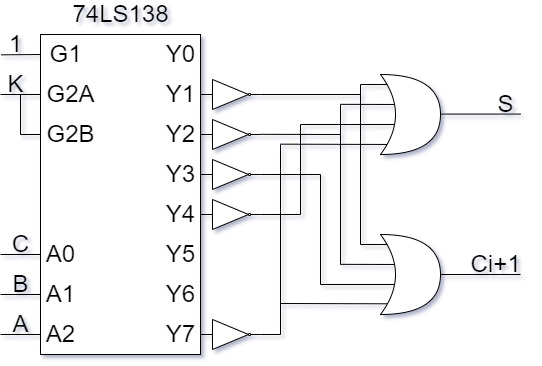
\includegraphics[width=0.8\textwidth]{image/electrical_8.png}\end{center}
\end{minipage}
\end{Answer}

\begin{question}{}{}
  4-17 Coding in Verilog using 74LS238.
\end{question}
\begin{Answer}
\begin{verilogcode}[caption={Verilog: 17}]
module adder_74283(
    input [3:0] A,
    input [3:0] B,
    input Cin,
    output [3:0] Sum,
    output Cout
);
assign {Cout, Sum} = A + B + Cin;
endmodule
module eight_bit_adder(
    input [7:0] num1,
    input [7:0] num2,
    output [7:0] result,
    output carry_out
);
    wire carry_intermediate;
    adder_74283 lower_bits(
        .A(num1[3:0]),
        .B(num2[3:0]),
        .Cin(1'b0),
        .Sum(result[3:0]),
        .Cout(carry_intermediate)
    );
    adder_74283 upper_bits(
        .A(num1[7:4]),
        .B(num2[7:4]),
        .Cin(carry_intermediate),
        .Sum(result[7:4]),
        .Cout(carry_out)
    );
endmodule
\end{verilogcode}

\begin{center}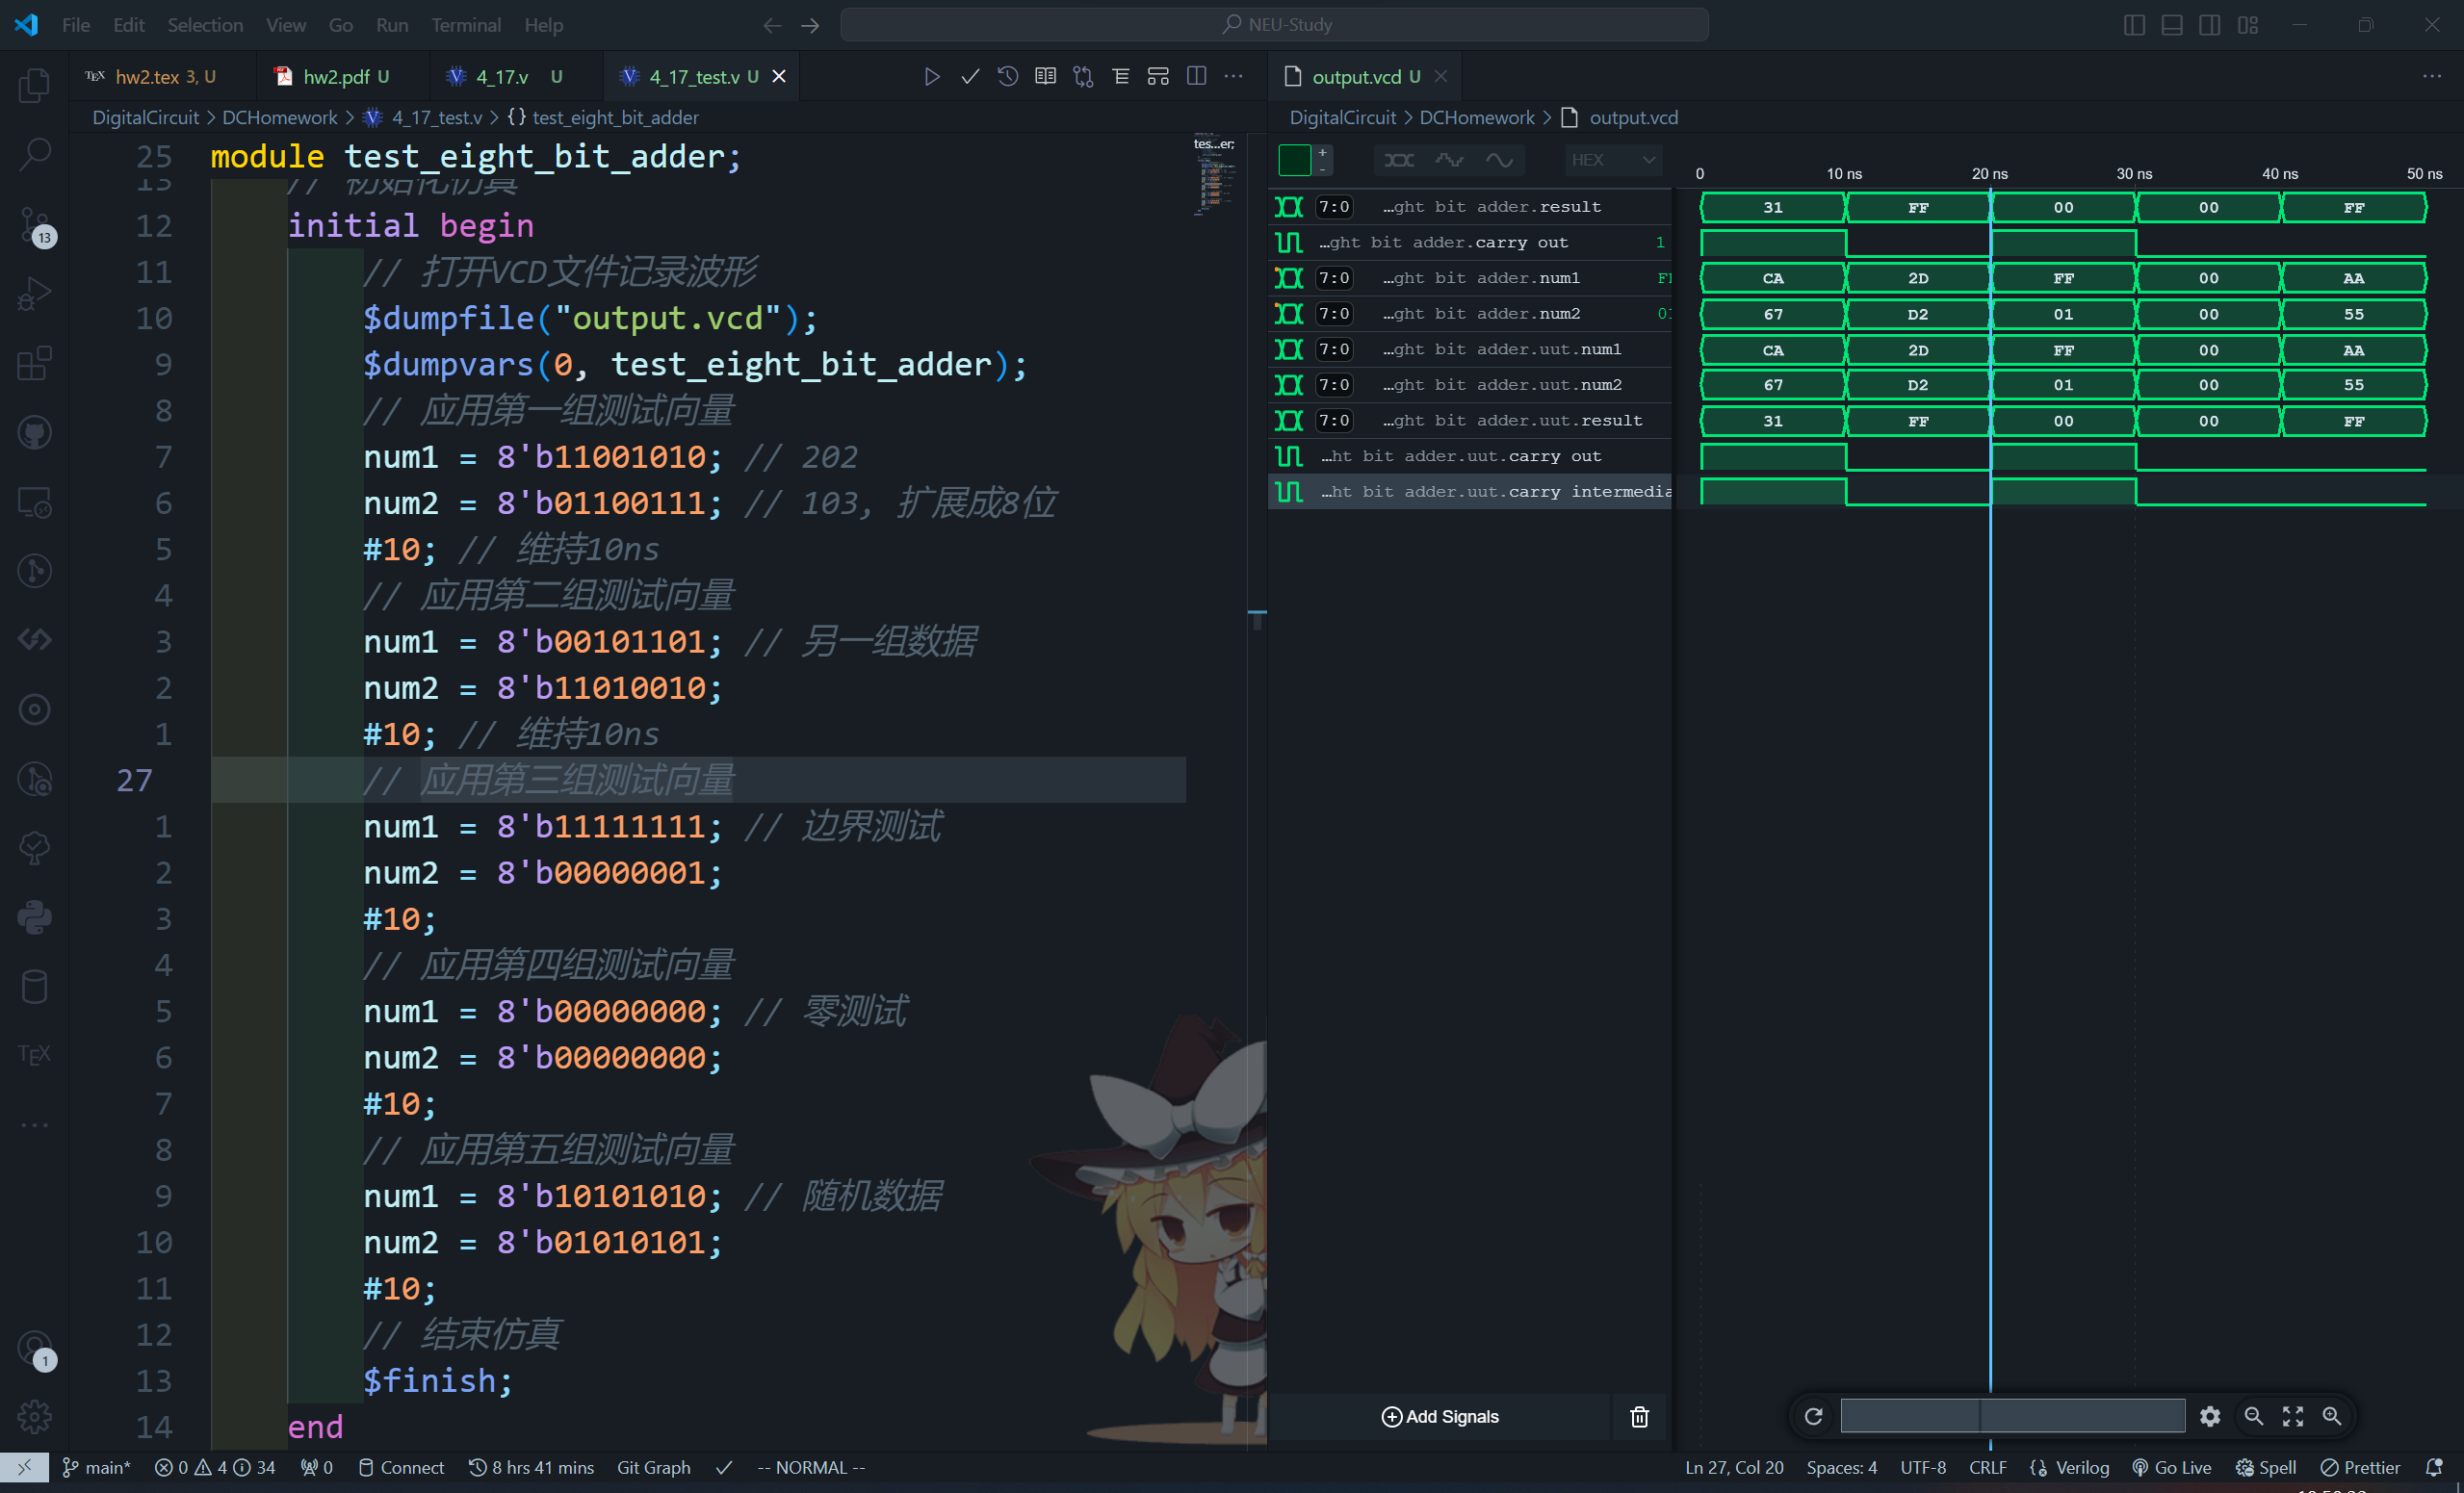
\includegraphics[width=1\textwidth]{image/electrical_9.png}\end{center}
\end{Answer}

得到的波形图如下：

\begin{question}{}{}
  4-18 Design Circuit using 74LS85.
\end{question}
\begin{Answer}
易得，电路图如下：

\begin{center}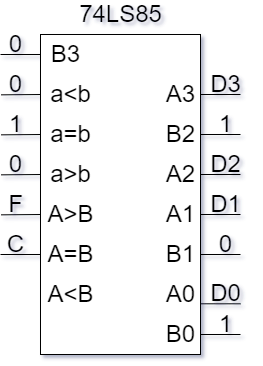
\includegraphics[width=0.2\textwidth]{image/electrical_10.png}\end{center}
\end{Answer}
\begin{question}{}{}
  4-19 Design Circuit using 74LS151.
\end{question}
\begin{Answer}
\noindent\begin{minipage}{0.5\textwidth}
\begin{center}\begin{tabular}{|c|c|c|c|c|}\hline
A & B & C & D & F \\ \hline
0 & 0 & 0 & 0 & 1 \\ \hline
0 & 0 & 0 & 1 & 0 \\ \hline
0 & 0 & 1 & 0 & 0 \\ \hline
0 & 0 & 1 & 1 & 1 \\ \hline
0 & 1 & 0 & 0 & 0 \\ \hline
0 & 1 & 0 & 1 & 1 \\ \hline
0 & 1 & 1 & 0 & 1 \\ \hline
0 & 1 & 1 & 1 & 0 \\ \hline
1 & 0 & 0 & 0 & 0 \\ \hline
1 & 0 & 0 & 1 & 1 \\ \hline
1 & 0 & 1 & 0 & 1 \\ \hline
1 & 0 & 1 & 1 & 0 \\ \hline
1 & 1 & 0 & 0 & 1 \\ \hline
1 & 1 & 0 & 1 & 0 \\ \hline
1 & 1 & 1 & 0 & 0 \\ \hline
1 & 1 & 1 & 1 & 1 \\ \hline
\end{tabular}\end{center}
\end{minipage}\begin{minipage}{0.4\textwidth}
\begin{center}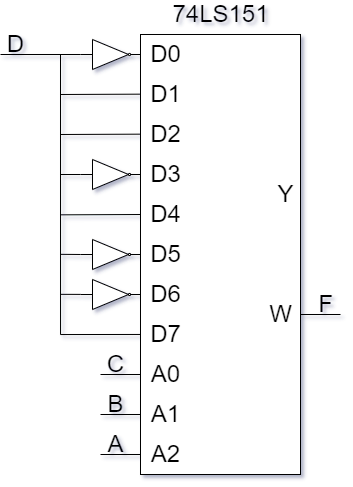
\includegraphics[width=1\textwidth]{image/electrical_11.png}\end{center}
\end{minipage}
\end{Answer}

\begin{question}{}{}
  4-21 Reading code and draw logic circuit and draw truth tables.
\end{question}
\begin{Answer}
\noindent\begin{minipage}{0.5\textwidth}
\quad\quad 功能为偶校验。

\begin{center}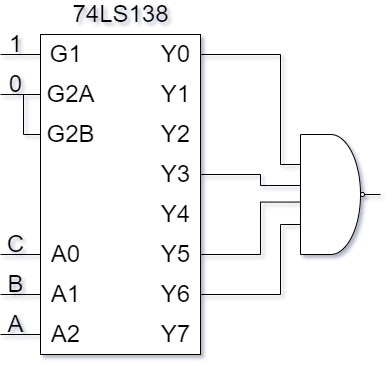
\includegraphics[width=0.5\textwidth]{image/electrical_12.png}\end{center}
\end{minipage}\begin{minipage}{0.5\textwidth}
\begin{center}\begin{tabular}{|c|c|c|c|}\hline
A & B & C & F \\ \hline
0 & 0 & 0 & 1 \\ \hline
0 & 0 & 1 & 0 \\ \hline
0 & 1 & 0 & 0 \\ \hline
0 & 1 & 1 & 1 \\ \hline
1 & 0 & 0 & 0 \\ \hline
1 & 0 & 1 & 1 \\ \hline
1 & 1 & 0 & 1 \\ \hline
1 & 1 & 1 & 0 \\ \hline
\end{tabular}\end{center}
\end{minipage}
\end{Answer}

\begin{question}{}{}
  4-22 Which number?
\end{question}
\begin{Answer}
\begin{center}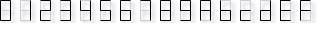
\includegraphics[width=1\textwidth]{image/electrical_13.png}\end{center}
\end{Answer}
\begin{flushright}\begin{tabular}{rl}
  姓名: & 李俊洁\\
  班级: & 计算机2204 \\
  学号: & 20225443 \\
  课程: & 数字逻辑与数字系统 \\
  日期: & April 26, 2024 \\
  制作: & \LaTeX \\
  & 感谢您的批阅！
\end{tabular}\end{flushright}
\end{document}